\documentclass[letter,12pt]{article}
\usepackage[utf8]{inputenc}
\usepackage{fullpage}
\usepackage{graphicx}
\usepackage{datetime}
\usepackage{indentfirst}

\newdateformat{mydate}{\THEDAY\space \shortmonthname[\THEMONTH] \THEYEAR}

\title{Switched LANs Lab Report}
\author{Sam Harkness}
\date{\mydate\today}

\begin{document}

%\maketitle

\begin{flushleft}
	\begin{tabular}{l l}
		To: & Prof. Richard Wolff \\
		From: & Sam Harkness \\
		Regarding: & Ethernet Lab Report \\
		Date: & \mydate\today
	\end{tabular}
\end{flushleft}



\begin{abstract}
	The objective of this lab is to demonstrate the operation of the Ethernet network. 6 scenarios were created for this project, all based on an Ethernet bus with 30 workstations.
	\begin{enumerate}
		\item The first 4 scenarios only differentiate on the rate that packets are generated.
		\item Coax\_Q3 has only 15 workstations instead of 30.
		\item Coax\_Q4 uses a reduced packet size of 512, instead of 1024 bytes.
	\end{enumerate}
\end{abstract}

\section{Question 1:}
	The throughput of the system increases until approximately 1000 packets/sec are send, then begins decreasing again.  This is due to the Ethernet bus architecture.  A node waits until the bus is open (free of communications) before it initiates its own transfer.  This unstructured approach to sharing a common medium works well for small numbers of nodes or small amounts of traffic, but begins to bog down when many nodes are attempting to communicate or there is a large amount of traffic.

	\begin{figure}[h!]
		\centering
			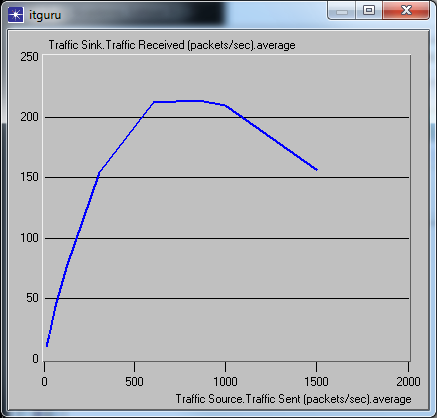
\includegraphics[scale=.6]{Throughput.png}
		\caption{Throughput}
		\label{Throughput}
	\end{figure}
	
\pagebreak

\section{Question 2:}
	As you can see in Figures~\ref{Collision_Count} and \ref{Q2_Traffic_Received}, scenario Coax\_Q2c has far more collisions than the other two scenarios, due to the increased rate of packets being sent.  However, it also has an increased number of packets received until near the end of the simulation.  This is due to the congestion of the bus overcoming it's throughput.
	
	\begin{figure}[h!]
		\centering
			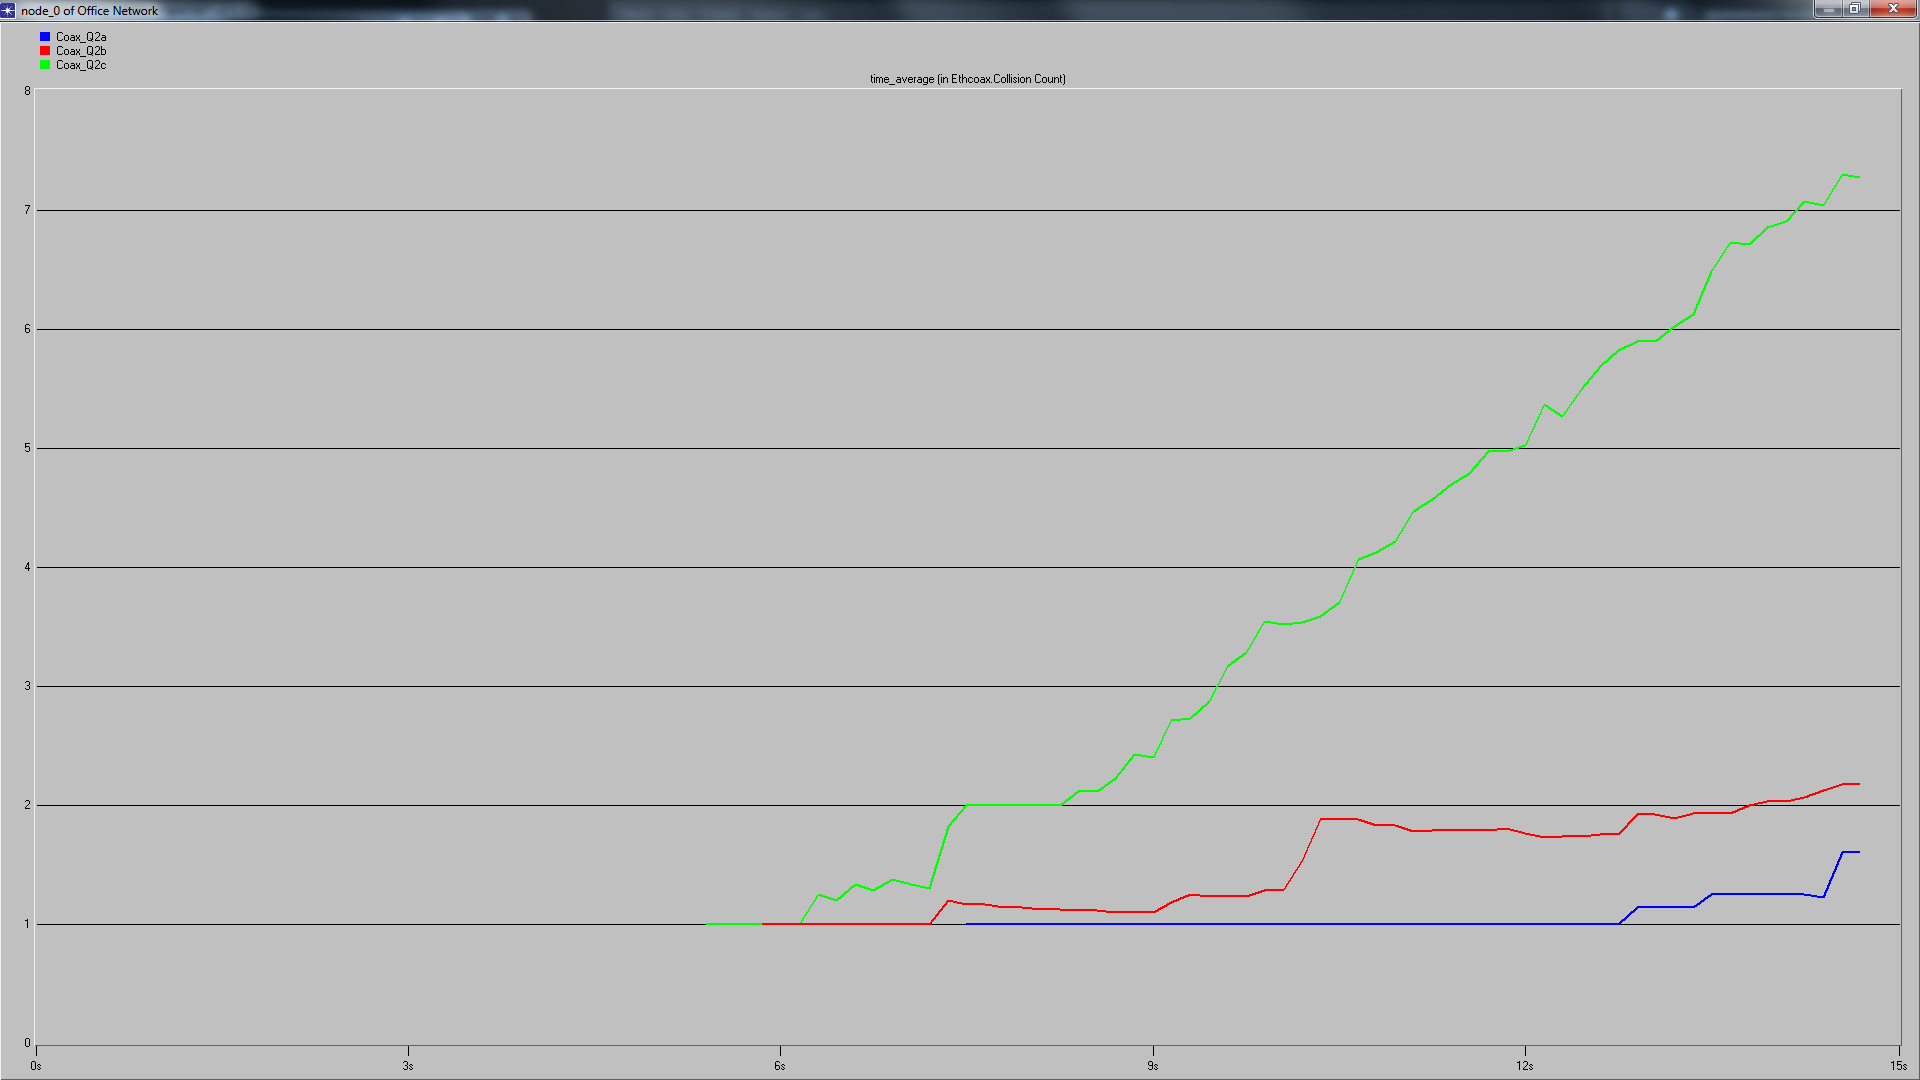
\includegraphics[width=.8\textwidth]{Collision_Count.png}
		\caption{Collision Count}
		\label{Collision_Count}
	\end{figure}
	
	\begin{figure}[h!]
		\centering
			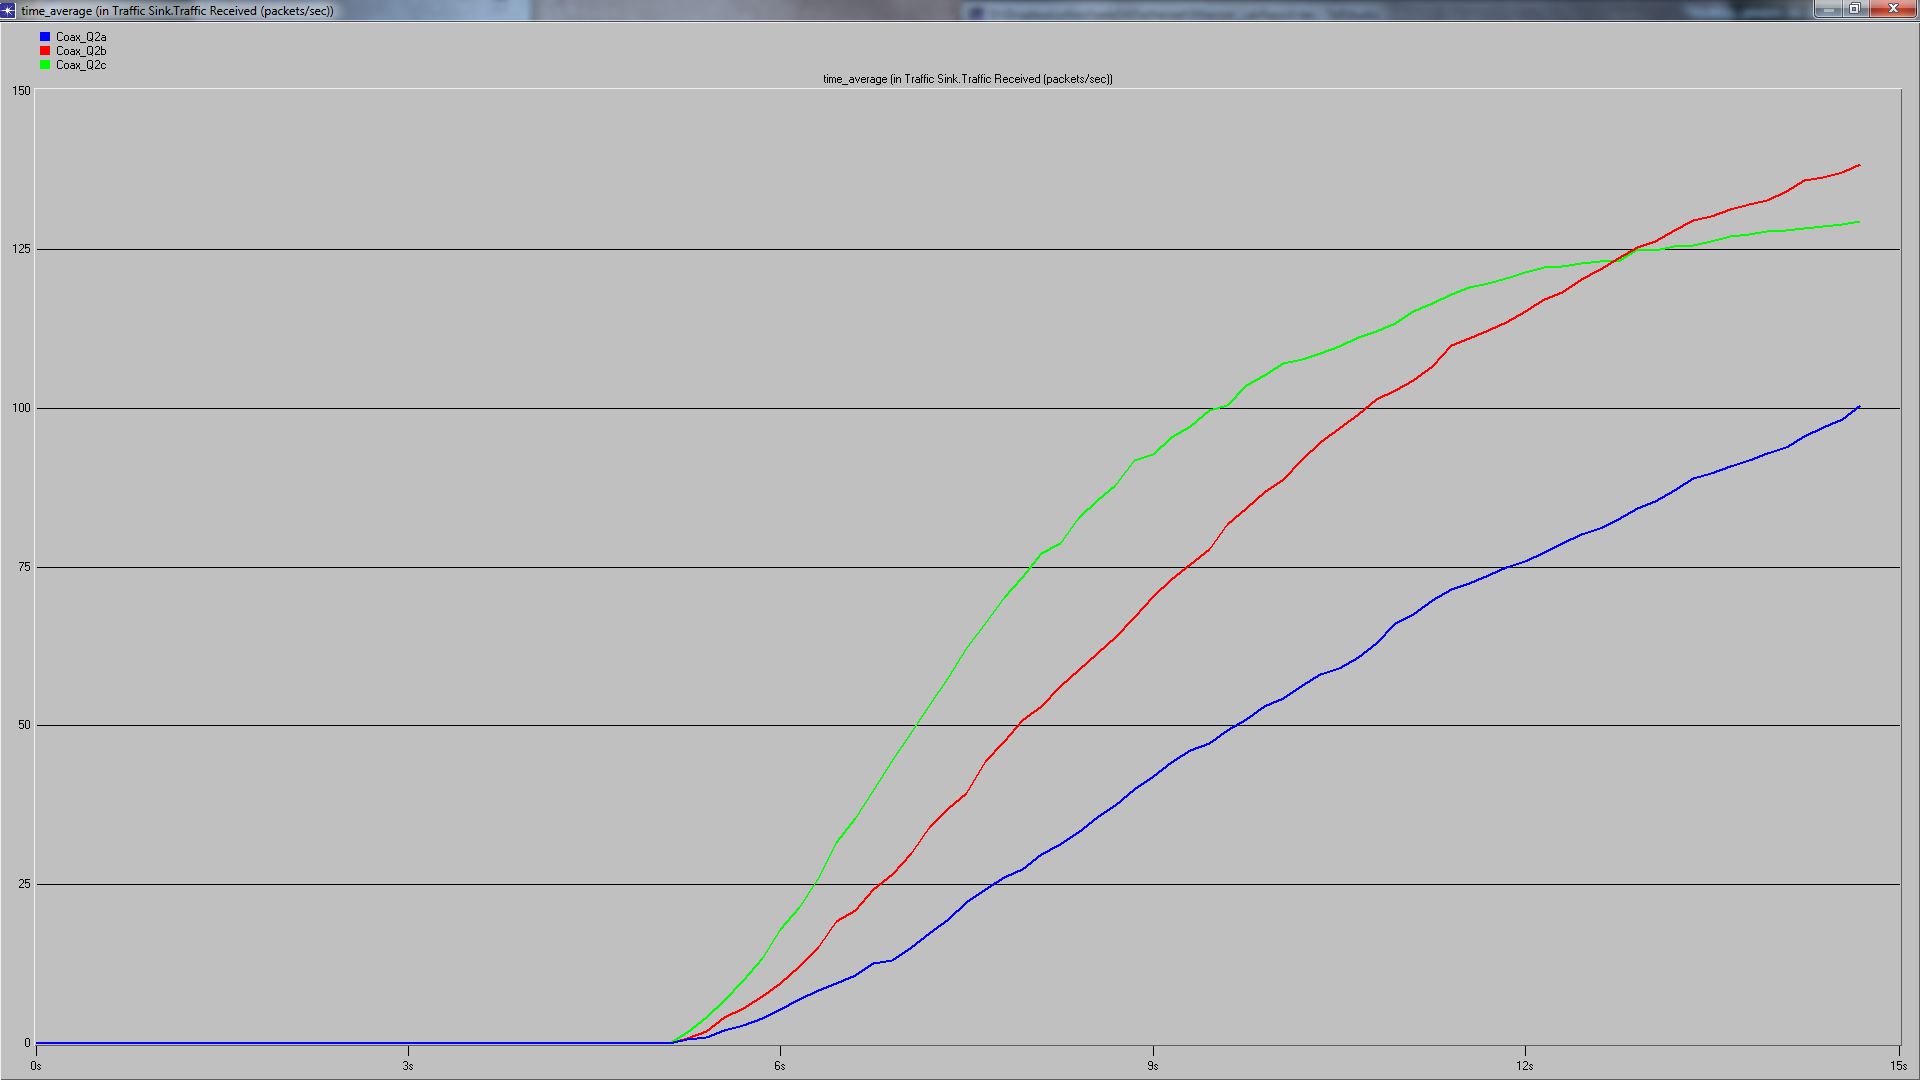
\includegraphics[width=.8\textwidth]{Q2_Traffic_Received.png}
		\caption{Traffic Received}
		\label{Q2_Traffic_Received}
	\end{figure}
		
\pagebreak

\section{Question 3:}
	Figure~\ref{Q3} shows the collision count of the 15 nodes vs 30 nodes.  Obviously, fewer nodes means fewer collisions.
	
	\begin{figure}[h!]
		\centering
			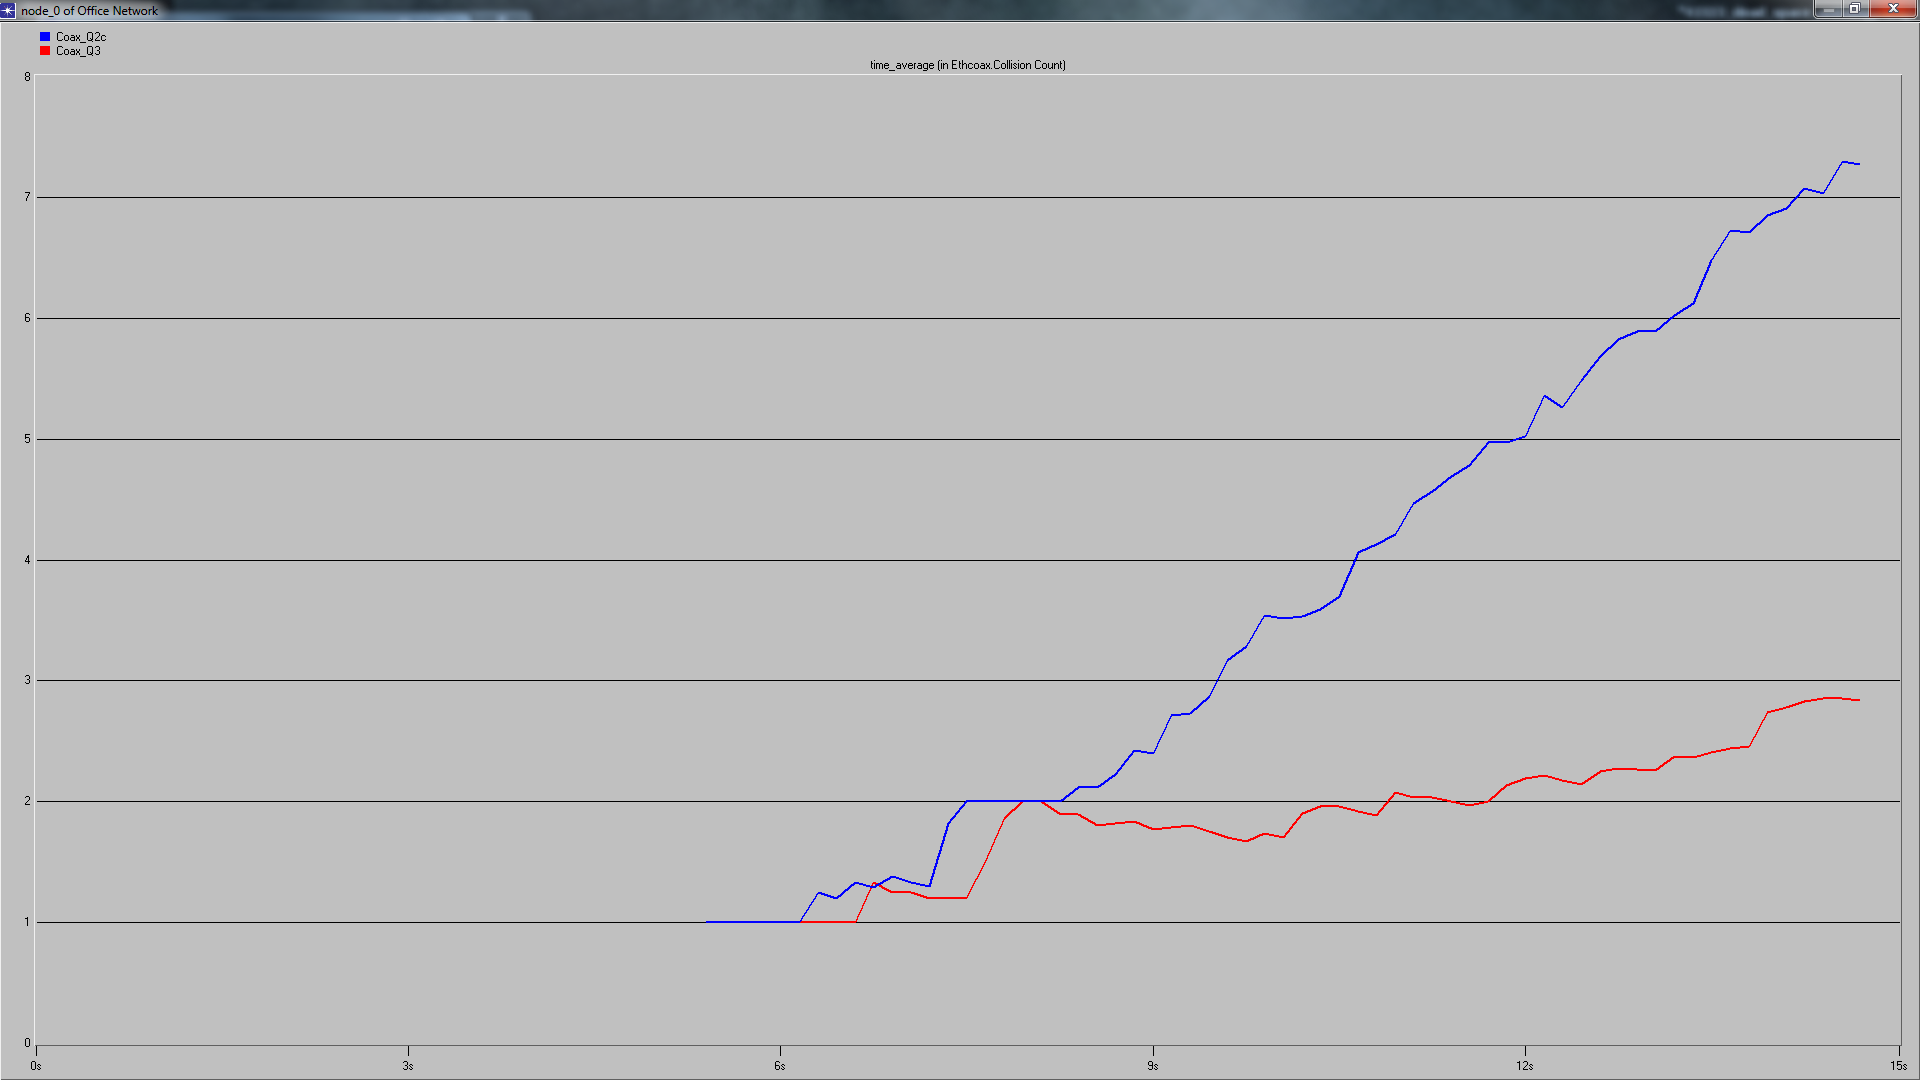
\includegraphics[width=.9\textwidth]{Q3.png}
		\caption{Collision Count of 15 nodes vs 30 nodes}
		\label{Q3}
	\end{figure}

\pagebreak

\section{Question 4:}
For this question, 2 scenarios were used, one with packet size of 1024 bytes, and one with 512 bytes.  Figure~\ref{Packets_per_Sec} shows that having a smaller packet size increases your packets per second, but Figure~\ref{Bits_per_Sec} shows that using a smaller packet size decreases the bit-rate of the system.

	\begin{figure}[h!]
		\centering
			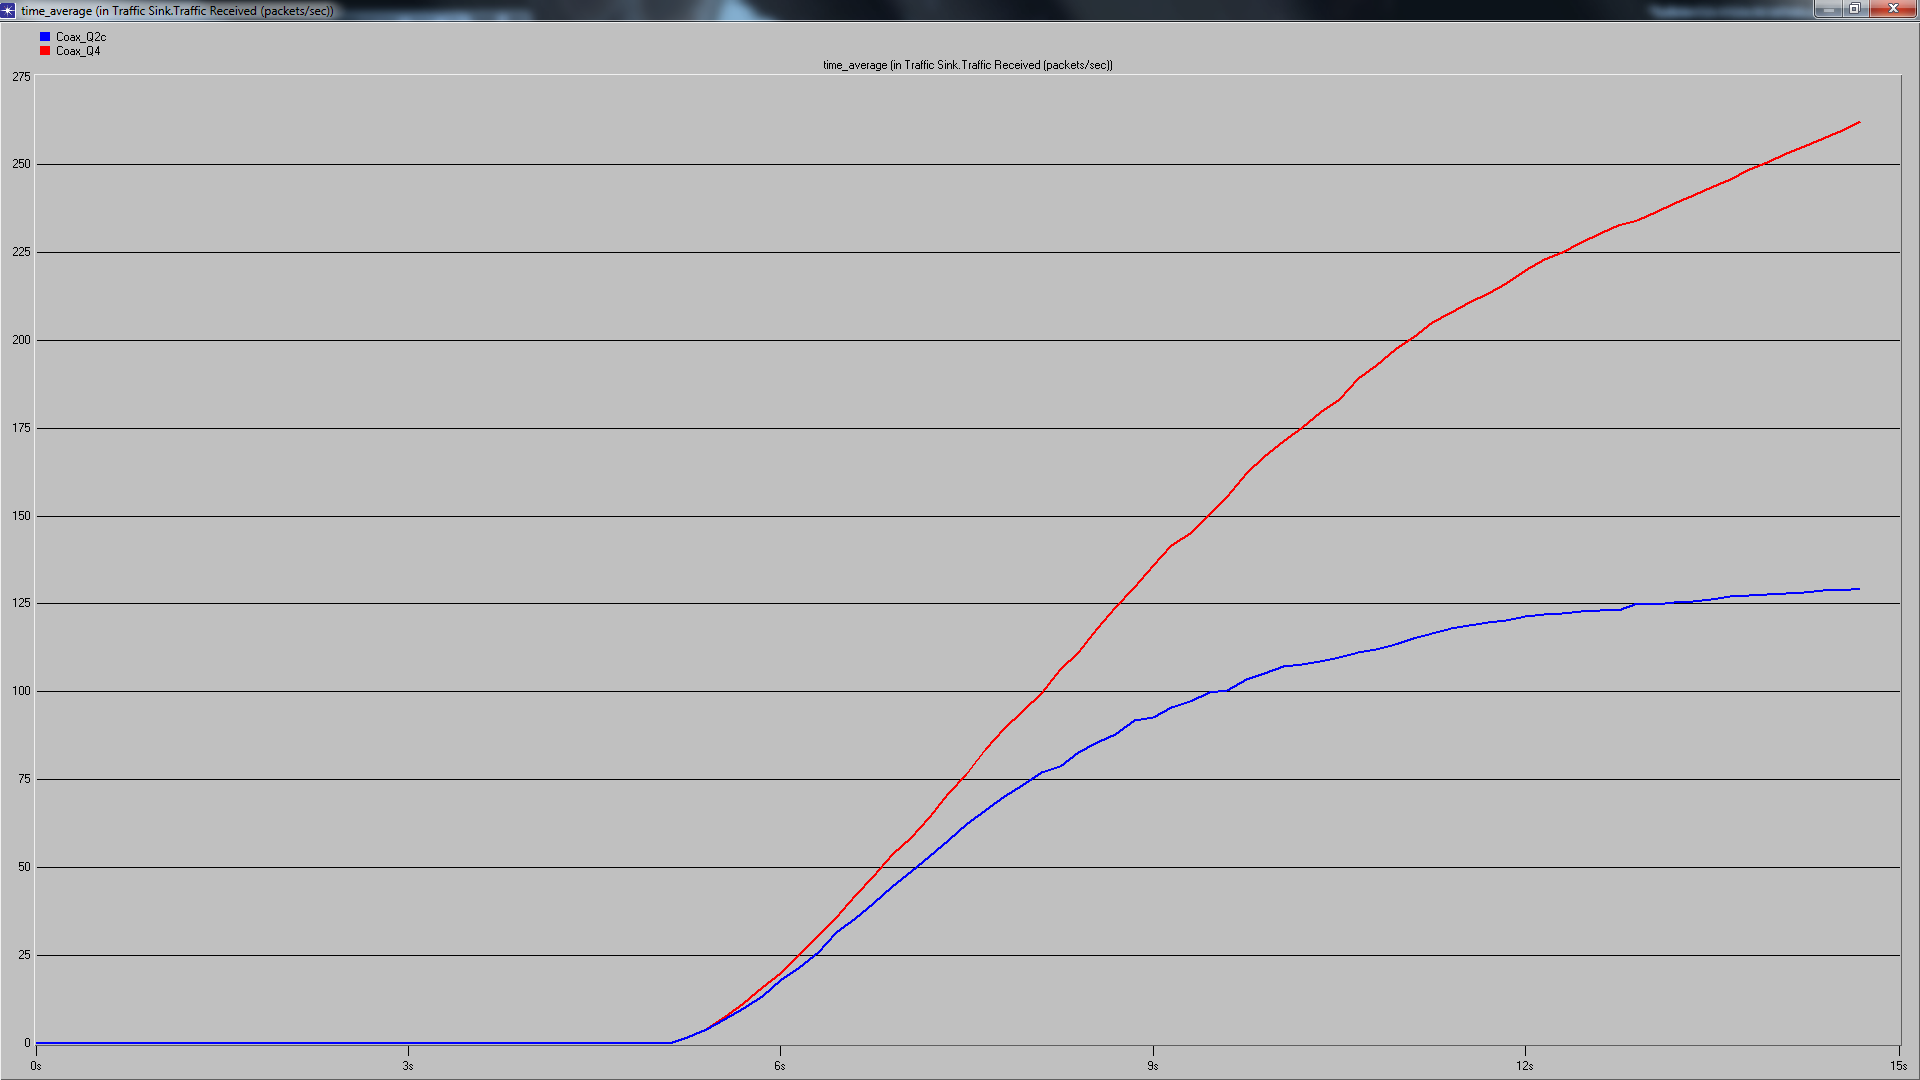
\includegraphics[width=.8\textwidth]{Packets_per_Sec.png}
		\caption{Packets per Second}
		\label{Packets_per_Sec}
	\end{figure}
	
	\begin{figure}[h!]
		\centering
			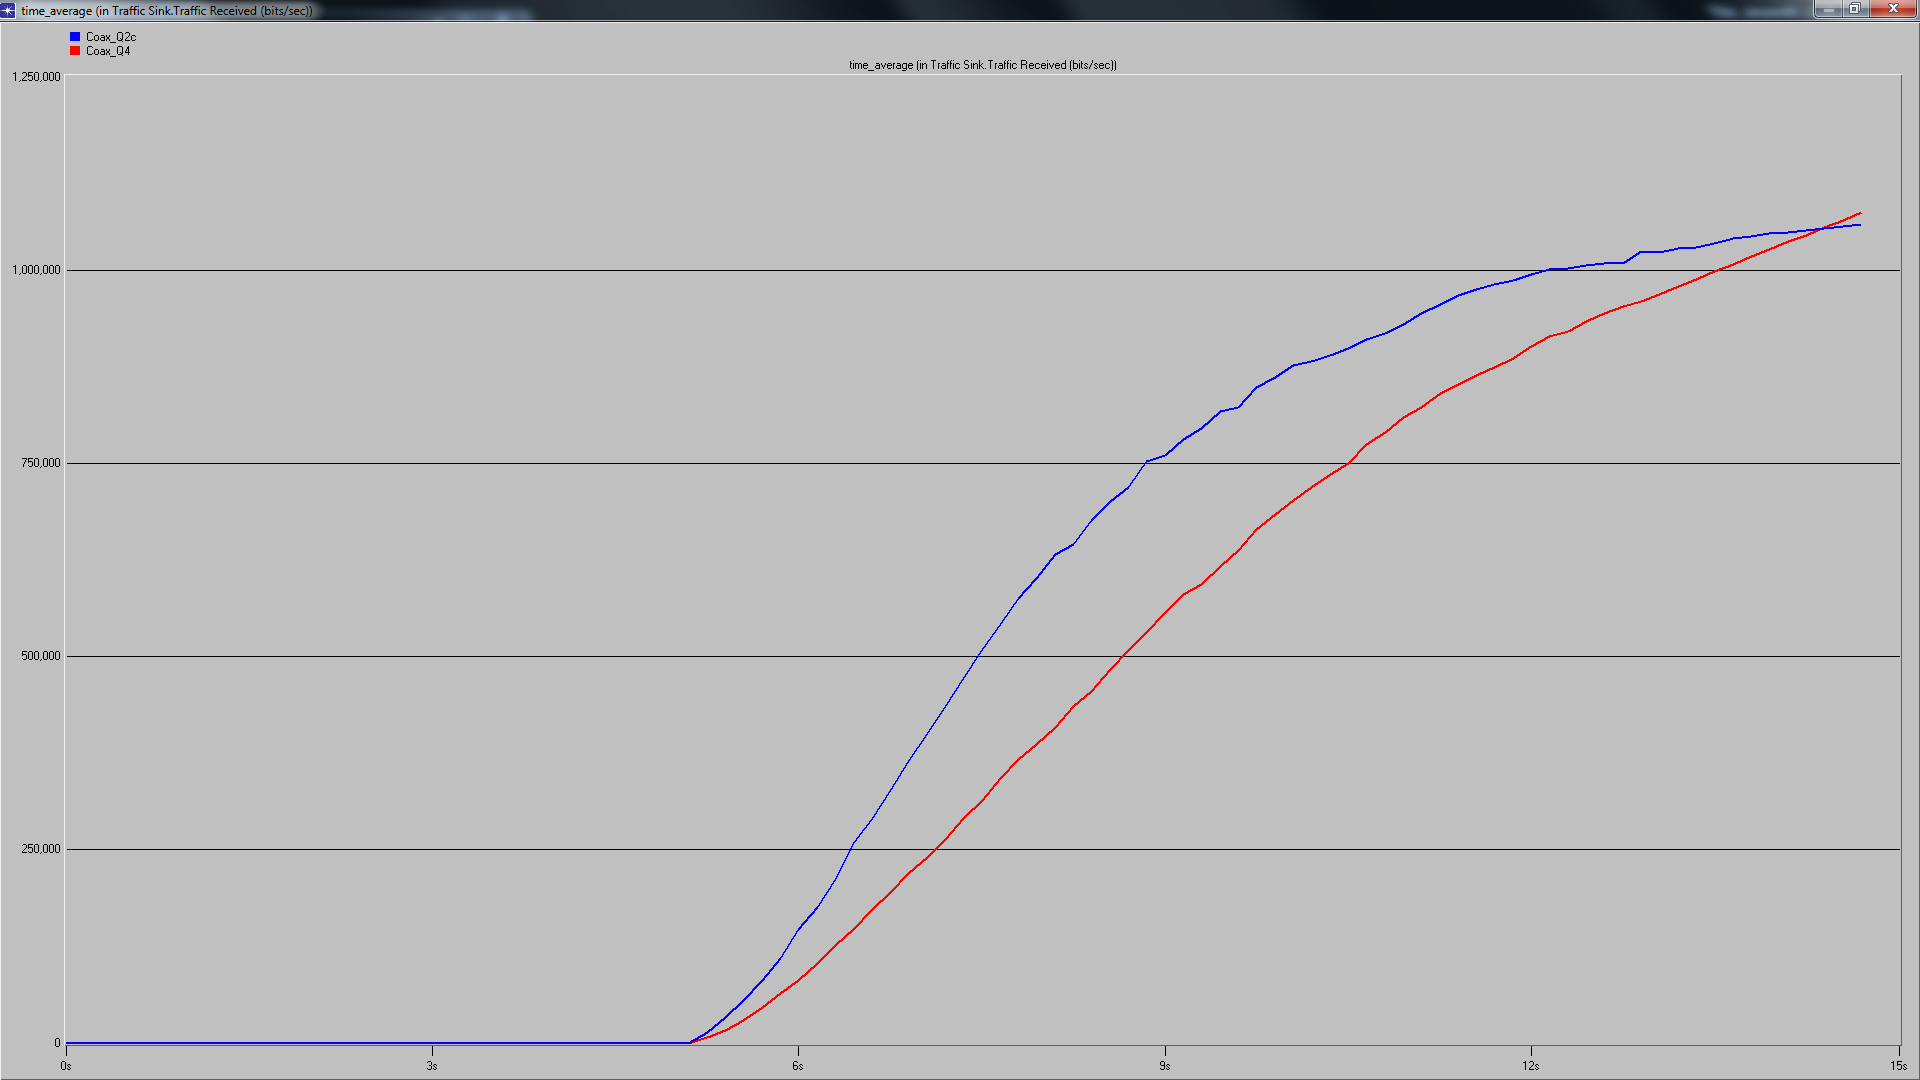
\includegraphics[width=.8\textwidth]{Bits_per_Sec.png}
		\caption{Bits per Second}
		\label{Bits_per_Sec}
	\end{figure}
	
\end{document}
